\section{Audit Rubric}
\label{app:rubric}

\subsection{Grading procedure}

Each audit grades one agent's attempt at one paper's central claim. The
auditor receives the claim with its pinned match target, a manifest of the run
bundle, and the frozen rubric text (Figure~\ref{lst:rubric-text}), and
it explores the bundle with the tools of Table~\ref{tab:audit-tools}. It places the run in the highest quality band the cited evidence meets,
then applies an integrity adjustment. The rubric
sets a low-score prior, so a run with no evidence scores low, and a printed number is not treated as verified.

\begin{table}[ht]
\centering
\footnotesize
\renewcommand{\arraystretch}{1.15}
\begin{tabular}{@{}l>{\raggedright\arraybackslash}p{10.6cm}@{}}
\toprule
Tool & Function and limits \\
\midrule
\texttt{list\_run\_files} & Lists files and directories in the run bundle,
optionally recursive. At most 200 entries, flagged when truncated. Prunes the
\texttt{.git}, \texttt{\_\_pycache\_\_}, \texttt{.venv}, and
\texttt{node\_modules} subtrees. \\
\texttt{read\_run\_file} & Reads one text file by relative path. Default cap
40{,}000 characters, maximum 200{,}000, flagged when truncated. \\
\texttt{bash} & Runs one shell command with the run bundle as the working
directory. Timeout 60\,s, after which the whole process group is killed.
Returns stdout, stderr, and the exit code. \\
\texttt{write\_run\_file} & Writes a new text file of up to 200{,}000 characters
into the bundle, such as a re-scoring script to run with \texttt{bash} and cite.
Refuses to overwrite an existing file, so agent artifacts stay intact. \\
\bottomrule
\end{tabular}
\caption{The four run-directory tools available to the auditor, with the
function and limits of each.}
\label{tab:audit-tools}
\end{table}

\subsection{Score scale and verdicts}

Table~\ref{tab:rubric} lists the score bands and the verdict each score maps
to. A score of 1 becomes \texttt{unverifiable} when the auditor also reports
that it found no evidence the code ran. We froze the rubric text on 2026-07-16,
three days after the dataset freeze, and every pinned-auditor grade in this
paper was produced after that date. An agent that reports it could not obtain
a required artifact, such as weights or a dataset, gets no credit for that
report. We had already removed every paper with a missing artifact from the
frozen split (Appendix~\ref{app:construction}), so such a report is a failure
of the run, and the auditor scores what the run did. If the auditor believes
the artifact is missing, it says so in \texttt{methodology\_notes} so that we
can recheck the paper.

{\small
\begin{longtable}{@{}c l >{\raggedright\arraybackslash}p{6.14cm} l@{}}
\toprule
Score & Band & Conditions & Verdict \\
\midrule
\endfirsthead
\multicolumn{4}{@{}l}{\footnotesize\itshape Table~\ref{tab:rubric}, continued.} \\[3pt]
\toprule
Score & Band & Conditions & Verdict \\
\midrule
\endhead
\midrule
\endfoot
\bottomrule
\noalign{\vskip 6pt}
\caption{The frozen audit rubric, with the conditions for each band and the
verdict derived from each score.}
\label{tab:rubric} \\
\endlastfoot
10 & Faithful, exact & Right experiment executed, C1 criterion met, no flags,
correct protocol, split, and scale; a stochastic metric seed-fixed or averaged.
& \texttt{reproduced} \\
9 & Faithful, single draw & As 10, with one unseeded draw of a stochastic metric
that still lands inside the bar. & \texttt{reproduced} \\
8 & Minor caveats & C1 criterion met with sound provenance; low-severity flags
only, or one medium flag whose evidence shows the deviation does not change the
measured quantity. The bar is never loosened at grade time. & \texttt{reproduced} \\
\midrule
7 & Near-reproduction & The authors' own pipeline, clean provenance, honest, and
the result lands just outside the bar, or inside it with an unresolved protocol
deviation, or all but one arm of a multi-part claim is met. & \texttt{partial} \\
6 & Clear partial & The right quantity executed with sound provenance, and the
result clearly misses the bar, or the pinned bar is mis-specified and the agent
reproduced the reproducible sibling quantity. & \texttt{partial} \\
\midrule
5 & Honest off-target & No authors' evaluation pipeline existed, so the agent
reconstructed the protocol in good faith, ran the whole evaluation, disclosed
the result, and it diverged from the target. & \texttt{not\_reproduced} \\
4 & Weak attempt & Executed but substantially off, with a large
non-cheating deviation, underpowered coverage, or an unvalidated
reimplementation. & \texttt{not\_reproduced} \\
3 & Killed before the number & Cited evidence shows the claim's own experiment
underway with progress toward the pinned metric and clean provenance, and
resources killed it before any valid number existed. The shortfall is reported
honestly. & \texttt{not\_reproduced} \\
2 & Failed execution & Code ran but foundered before the claim's experiment was
underway, or addressed the wrong task, reported honestly. &
\texttt{not\_reproduced} \\
1 & Non-attempt & No execution evidence, a bundle too thin to grade, or no
checkable target, and the run does not misrepresent itself. &
\texttt{unverifiable} \\
0 & Integrity break & Any high-severity anti-cheat flag, a report whose verdict
contradicts its own evidence, a proxy substituted into the target slot, or a
retrieved benchmark answer the graded value runs through. &
\texttt{disqualified} \\
\end{longtable}
}

Figure~\ref{fig:score-dist} shows how the 372 graded runs fall across the scale.
The distribution has a mode at 4, where a run executes something the auditor can
grade and lands well short of the bar, and a second at 0, where an integrity
flag zeroes the score.

\begin{figure}[ht]
\centering
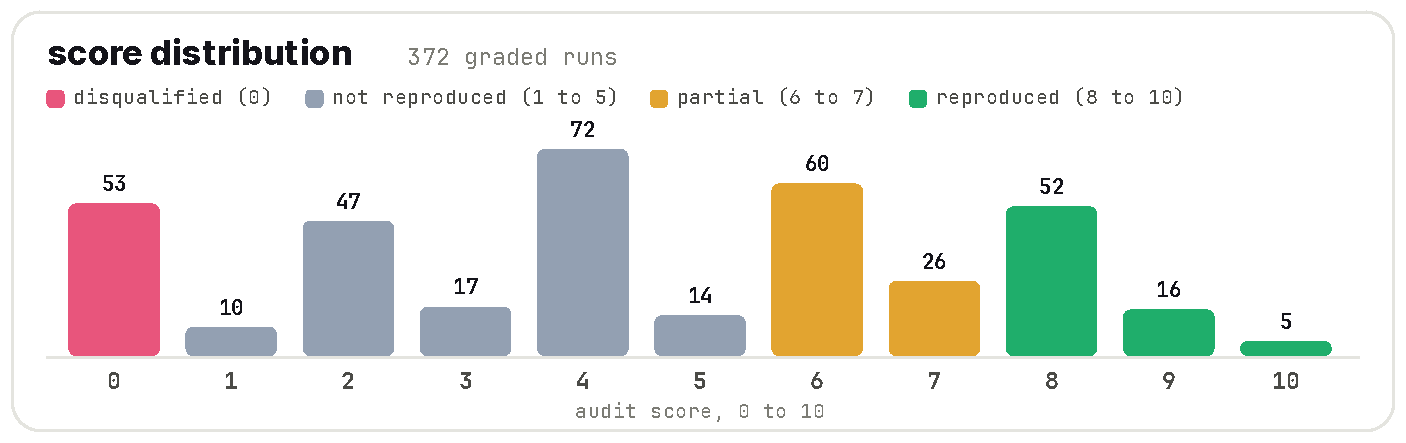
\includegraphics[width=\textwidth]{figures/score_distribution}
\caption{Audit scores over the 372 graded runs, colored by the verdict bands of
Table~\ref{tab:rubric}.}
\label{fig:score-dist}
\end{figure}

\subsection{Deterministic verdict derivation}
\label{app:rubric-finalizer}

\codefile[lst:audit-finalizer]{Python}{Verdict derivation code}{prompts/audit_finalizer.py}
